\documentclass[11pt]{amsart}

% ── Packages ──────────────────────────────────────────────────────────────
\usepackage[margin=1in]{geometry}
\usepackage{amsmath,amssymb,amsthm}
\usepackage{graphicx}
\usepackage{booktabs}
\usepackage{hyperref}
\usepackage{microtype}
\usepackage{enumitem}
\usepackage{xcolor}
\usepackage{float}
\usepackage{caption}
\usepackage{subcaption}
\usepackage{mathtools}
\usepackage{tikz}
\usepackage{algorithm}
\usepackage{algpseudocode}
\usepackage[numbers,sort&compress]{natbib}

% ── Theorem environments ──────────────────────────────────────────────────
\newtheorem{theorem}{Theorem}[section]
\newtheorem{lemma}[theorem]{Lemma}
\newtheorem{proposition}[theorem]{Proposition}
\newtheorem{corollary}[theorem]{Corollary}
\newtheorem{conjecture}[theorem]{Conjecture}
\theoremstyle{definition}
\newtheorem{definition}[theorem]{Definition}
\newtheorem{example}[theorem]{Example}
\theoremstyle{remark}
\newtheorem{remark}[theorem]{Remark}
\newtheorem{observation}[theorem]{Observation}

% ── Macros ────────────────────────────────────────────────────────────────
\newcommand{\R}{\mathbb{R}}
\newcommand{\C}{\mathbb{C}}
\newcommand{\Z}{\mathbb{Z}}
\newcommand{\Nat}{\mathbb{N}}
\newcommand{\half}{\tfrac{1}{2}}
\newcommand{\abs}[1]{\lvert #1 \rvert}
\newcommand{\norm}[1]{\lVert #1 \rVert}
\newcommand{\re}{\operatorname{Re}}
\newcommand{\im}{\operatorname{Im}}
\DeclareMathOperator{\ord}{ord}

\hypersetup{
  colorlinks=true,
  linkcolor=blue!70!black,
  citecolor=blue!70!black,
  urlcolor=blue!70!black
}

% ══════════════════════════════════════════════════════════════════════════
\title[The $\omega$-Class Decomposition]{The $\omega$-Class Decomposition of Dirichlet Polynomials:\\
A New Framework for the Lindel\"of Hypothesis}

\author{David Alejandro Trejo Pizzo}
\thanks{Independent Researcher. \texttt{dtrejopizzo@gmail.com}}

\begin{document}
\begin{abstract}
We introduce the \emph{$\omega$-class decomposition}, a partition of the
standard Dirichlet polynomial $D(t;N) = \sum_{n \le N} n^{-1/2-it}$
into sub-sums $S_k(t;N)$ indexed by $\omega(n) = k$, the number of
distinct prime factors.  We prove four unconditional theorems bounding
the amplification ratio $(1+r) = |D|^2 / \sum_k |S_k|^2$, culminating
in a reduction: a uniform pointwise bound
$B(N) = \max_{t,k} |S_k(t;N)|^2 \le C_\varepsilon N^\varepsilon$
on the individual class sums, for every $\varepsilon > 0$, \emph{implies}
the Lindel\"of Hypothesis.  We stress that this is a one-directional
\emph{sufficient} condition: because $B(N)$ controls each $\omega$-class
separately, whereas the Lindel\"of Hypothesis constrains only the full
sum~$D$, the bound $B(N)\le N^\varepsilon$ is plausibly \emph{strictly
stronger} than LH and is not known to follow from it.  We prove a conditional \emph{Master Theorem}
linking $B(N) \le N^\alpha$ to the bound
$|\zeta(\half + it)| \ll t^{\alpha/2 + \varepsilon}$
via the Approximate Functional Equation.
Extensive computation at $N \in \{10^4, 5 \times 10^4, 10^5, 1.5 \times 10^5\}$
reveals: (i)~the empirical exponent $\alpha_B = \log B(N)/\log N$ decreases
from $0.428$ to $0.395$ in the $k{=}2$ regime;
(ii)~a dominance transition from $k{=}2$ (semiprimes) to $k{=}3$
(triprimes) occurs near $N \approx 10^5$, causing a reversal in
$\alpha_B$; (iii)~a phase resonance mechanism with Rayleigh statistic
$R \approx 0.92$ explains the hardness gap between large-sieve mean
bounds and observed maxima.  We formulate the open problem of
bounding $B(N)$ uniformly over all $\omega$-classes and discuss
connections to bilinear and multilinear exponential sum estimates.
Full reproduction code is provided.
\end{abstract}

\maketitle

% ══════════════════════════════════════════════════════════════════════════


\tableofcontents
\newpage

% ══════════════════════════════════════════════════════════════════════════
\section{Introduction}\label{sec:intro}
The Lindel\"of Hypothesis (LH) asserts that for every $\varepsilon > 0$,
\begin{equation}\label{eq:lindelof}
  \abs{\zeta(\half + it)} \ll_\varepsilon t^\varepsilon
  \qquad (t \to \infty).
\end{equation}
This would follow from the Riemann Hypothesis (RH), but the converse
is false: LH is strictly weaker than RH.
Despite a century of effort, the best unconditional bound remains
subconvex: $\abs{\zeta(\half+it)} \ll t^{13/84+\varepsilon}$
(Bourgain~\cite{bourgain2017}).

Our approach begins with the observation that the Dirichlet polynomial
\begin{equation}\label{eq:D_def}
  D(t;N) = \sum_{n=2}^{N} n^{-1/2 - it}
\end{equation}
approximates $\zeta(\half+it)$ for $N \sim t$ (via the Approximate
Functional Equation, Theorem~\ref{thm:master}).  We decompose $D$
by the arithmetic function $\omega(n)$, the number of distinct prime
factors of~$n$:
\begin{equation}\label{eq:Sk_def}
  S_k(t;N) = \sum_{\substack{n \le N \\ \omega(n) = k}}
    n^{-1/2-it}, \qquad
  D(t;N) = \sum_{k=1}^{K_N} S_k(t;N),
\end{equation}
where $K_N = \max\{\omega(n) : 2 \le n \le N\}$.

The ratio between $|D|^2$ and the diagonal energy
$E = \sum_k |S_k|^2$ encodes the interference structure:
\begin{equation}\label{eq:1pr_def}
  1 + r(t;N) = \frac{|D(t;N)|^2}{E(t;N)}.
\end{equation}

Our main results are:
\begin{enumerate}[label=(\roman*)]
  \item \textbf{Amplification Bound} (Theorem~\ref{thm:CS}):
    $(1+r) \le K_N \le \lfloor \log_2 N \rfloor$, unconditionally.
  \item \textbf{Reduction} (Theorem~\ref{thm:reduction}):
    $|D|^2 \le K_N^2 \cdot B(N)$, reducing LH to bounding
    individual class sums.
  \item \textbf{Effective Class Count} (Theorem~\ref{thm:Kcount}):
    $K_N \sim \log N / \log\log N$.
  \item \textbf{Refined Bound} (Theorem~\ref{thm:refined}):
    $(1+r) \le (\sum_k \sqrt{p_k})^2$, 5--23\% tighter than~(i).
  \item \textbf{Master Theorem} (Theorem~\ref{thm:master}):
    If $B(N) \le N^\alpha$, then
    $|\zeta(\half+it)| \ll t^{\alpha/2+\varepsilon}$.
\end{enumerate}

\noindent
Theorems (i)--(iv) are unconditional.  Theorem~(v) is conditional
on a hypothesis about~$B(N)$ and uses the Approximate Functional Equation.

\medskip
\noindent\textbf{On the direction of the reduction.}
We emphasize at the outset that the chain Theorem~\ref{thm:reduction}
$\to$ Theorem~\ref{thm:master} is \emph{one-directional}:
$B(N)\le N^\varepsilon \Rightarrow \mathrm{LH}$.  The converse fails, or at
least is not available: $B(N)=\max_{t,k}|S_k|^2$ bounds each $\omega$-class
\emph{individually}, whereas LH bounds only the total $|D|\approx|\zeta|$,
which may remain small through cancellation \emph{between} classes even
when some $|S_k|$ is large (Proposition~\ref{prop:stronger}).  Thus
$B(N)\le N^\varepsilon$ is a \emph{sufficient} condition for LH that is
plausibly strictly stronger.  This is not a defect of the framework but its
content: it isolates the precise pointwise quantity whose control would
yield LH, and the computations below measure exactly how far that quantity
is from the required bound.

\medskip

\noindent\textbf{Computational findings.}
We compute $B(N)$ at four values of~$N$ up to $1.5 \times 10^5$ and
observe:
\begin{itemize}
  \item The empirical exponent $\alpha_B(N)$ \emph{decreases} in the
    semiprime-dominated regime ($N \le 10^5$), consistent with
    $\alpha_B \to 0$ as $N \to \infty$.
  \item A dominance transition $k^* = 2 \to k^* = 3$ occurs near
    $N \approx 10^5$, causing $\alpha_B$ to increase temporarily.
  \item The large-sieve inequality bounds the \emph{mean}
    $\langle |S_k|^2\rangle$ well, but the \emph{maximum} exceeds the
    mean by factors of 25--90 due to phase resonance.
\end{itemize}

\medskip

\noindent\textbf{Organization.}
Section~\ref{sec:setup} establishes notation.
Sections~\ref{sec:thm1}--\ref{sec:thm5} contain the five theorems
with complete proofs.  Section~\ref{sec:computation} presents
computational results.
Section~\ref{sec:resonance} analyzes the phase resonance mechanism.
Section~\ref{sec:discussion} discusses connections and open problems.
Appendix~\ref{app:code} provides reproduction code.

% ══════════════════════════════════════════════════════════════════════════
\section{Setup and Notation}\label{sec:setup}

Throughout, $N \ge 2$ is a positive integer and $t \in \R$.
We write $\omega(n)$ for the number of distinct prime factors of~$n$
(with $\omega(1) = 0$), and $\Omega(n)$ for the number counted with
multiplicity.  The notation $f \ll g$ and $f = O(g)$ are synonymous;
$f \ll_\varepsilon g$ means the implied constant depends on~$\varepsilon$.
We write $f \lesssim g$ to mean $f \ll_\varepsilon g \cdot N^\varepsilon$
(or $t^\varepsilon$) for every $\varepsilon > 0$.

\begin{definition}[Dirichlet polynomial and $\omega$-class sums]
\label{def:D_and_Sk}
Let $F$ be a completely multiplicative function with $|a_n| \le 1$.
Define:
\begin{align}
  D_F(t;N) &= \sum_{n=2}^{N} a_n \, n^{-1/2-it}, \label{eq:DF}\\
  S_k(t;N) &= \sum_{\substack{n \le N \\ \omega(n) = k}}
    a_n \, n^{-1/2-it}, \qquad k = 1, 2, \ldots, K_N. \label{eq:SkF}
\end{align}
For $\zeta$, we take $a_n = 1$ for all~$n$.
\end{definition}

\begin{definition}[Energy, cross-terms, amplification ratio]
\label{def:energy}
\begin{align}
  E(t;N) &= \sum_{k=1}^{K_N} |S_k(t;N)|^2, \label{eq:E}\\
  X(t;N) &= |D(t;N)|^2 - E(t;N)
    = 2 \sum_{j < k} \re\bigl(\overline{S_j} \, S_k\bigr), \label{eq:X}\\
  r(t;N) &= \frac{X(t;N)}{E(t;N)}, \qquad
  1 + r(t;N) = \frac{|D(t;N)|^2}{E(t;N)}. \label{eq:r}
\end{align}
\end{definition}

\begin{definition}[Maximum class-sum and empirical exponent]
\label{def:BN}
\begin{align}
  B(N) &= \max_{\substack{t \in [N/10, N] \\
    1 \le k \le K_N}} |S_k(t;N)|^2, \label{eq:BN}\\
  \alpha_B(N) &= \frac{\log B(N)}{\log N}. \label{eq:alphaB}
\end{align}
\end{definition}

The energy fractions are $p_k(t) = |S_k(t)|^2 / E(t)$, satisfying
$\sum_k p_k = 1$.

% ══════════════════════════════════════════════════════════════════════════
\section{Theorem 1: Amplification Bound}\label{sec:thm1}

\begin{theorem}[Cauchy--Schwarz Amplification Bound]\label{thm:CS}
For any completely multiplicative function $F$ with $|a_n| \le 1$,
any $N \ge 2$, and any $t \in \R$:
\begin{equation}\label{eq:CS_bound}
  1 + r_F(t;N) \le K_N.
\end{equation}
Moreover, $K_N \le \lfloor \log_2 N \rfloor$.
\end{theorem}

\begin{proof}
By the Cauchy--Schwarz inequality applied to $K_N$ complex numbers
$S_1, \ldots, S_{K_N}$:
\[
  \abs{\sum_{k=1}^{K_N} S_k}^2
  \le K_N \sum_{k=1}^{K_N} |S_k|^2,
\]
with equality if and only if all $S_k$ are proportional.
Dividing both sides by $E = \sum_k |S_k|^2$:
\[
  1 + r = \frac{|D|^2}{E}
  = \frac{|\sum_k S_k|^2}{\sum_k |S_k|^2}
  \le K_N.
\]

For the bound on $K_N$: every integer $n \ge 2$ satisfies
$n \ge \prod_{p \mid n} p \ge 2^{\omega(n)}$,
since each prime $p \ge 2$.  Therefore
$\omega(n) \le \log_2 n \le \log_2 N$,
giving $K_N \le \lfloor \log_2 N \rfloor$.
\end{proof}

\begin{remark}
The bound is tight in the sense that equality $(1+r) = K_N$
requires all $K_N$ class sums to have equal magnitude and aligned phases.
Computationally, we observe $\max_t(1+r) \approx 4.0$ at $N = 10^4$
(where $K_N = 5$), so the bound has roughly~20\% slack.
\end{remark}

% ══════════════════════════════════════════════════════════════════════════
\section{Theorem 2: Reduction to Class Sum Bounds}\label{sec:thm2}

\begin{theorem}[Reduction]\label{thm:reduction}
For any $N \ge 2$ and $t \in \R$:
\begin{equation}\label{eq:reduction}
  |D_F(t;N)|^2 \le K_N^2 \cdot
  \max_{1 \le k \le K_N} |S_k(t;N)|^2.
\end{equation}
\end{theorem}

\begin{proof}
From Theorem~\ref{thm:CS}:
$|D|^2 \le K_N \cdot E$.
Since $E = \sum_{k=1}^{K_N} |S_k|^2
\le K_N \cdot \max_k |S_k|^2$,
we obtain
$|D|^2 \le K_N \cdot (K_N \max_k |S_k|^2)
= K_N^2 \max_k |S_k|^2$.
\end{proof}

\begin{corollary}[Reduction to Lindel\"of]\label{cor:lindelof}
If for every $\varepsilon > 0$ there exists $C_\varepsilon$ such that
$B(N) \le C_\varepsilon N^\varepsilon$, then the Lindel\"of Hypothesis
holds.
\end{corollary}

\begin{proof}
This follows from Theorem~\ref{thm:reduction} combined with
Theorem~\ref{thm:master} below, setting $\alpha = \varepsilon$.
\end{proof}

\begin{proposition}[The reduction is sufficient, not equivalent]
\label{prop:stronger}
The implication of Corollary~\ref{cor:lindelof} is one-directional. If LH
holds then, for fixed~$k$ and $N\sim t$, the mean value satisfies
$\frac1T\int_0^T |S_k(\half+it;N)|^2\,dt \ll N^\varepsilon$ (a consequence
of the large sieve, Section~\ref{sec:discussion}); but the \emph{pointwise}
maximum $B(N)=\max_{t,k}|S_k|^2$ is not controlled by LH, since LH bounds
only $|D|=|\sum_k S_k|$ and a single class sum may be large while the total
is small through inter-class cancellation. Consequently $B(N)\le
N^\varepsilon$ implies, but is not implied by, LH; it is plausibly strictly
stronger. The gap between the mean (large-sieve--controlled) and the
maximum is quantified in Section~\ref{sec:resonance} (peak-to-mean ratios
of $25$--$90$).
\end{proposition}

% ══════════════════════════════════════════════════════════════════════════
\section{Theorem 3: Effective Class Count}\label{sec:thm3}

\begin{theorem}[Class Count]\label{thm:Kcount}
$K_N = \max\{\omega(n) : n \le N\}$ satisfies:
\begin{enumerate}[label=(\alph*)]
  \item $K_N \le \lfloor \log_2 N \rfloor$ \textup{(}exact\textup{)}.
  \item $K_N \sim \frac{\log N}{\log\log N}$ as $N \to \infty$
    \textup{(}asymptotic\textup{)}.
  \item The maximum is achieved by the largest primorial
    $P_m = p_1 p_2 \cdots p_m \le N$.
\end{enumerate}
\end{theorem}

\begin{proof}
Part~(a) is proven in Theorem~\ref{thm:CS}.

For~(c): among all $n \le N$ with $\omega(n) = m$, the smallest is the
$m$-th primorial $P_m = 2 \cdot 3 \cdot 5 \cdots p_m$, since replacing
any prime factor by a larger prime only increases~$n$.  Therefore
$K_N = \max\{m : P_m \le N\}$.

For~(b): by the Prime Number Theorem, $p_m \sim m \log m$, so
$\log P_m = \sum_{j=1}^m \log p_j \sim m \log m$.
Setting $\log P_m \approx \log N$ gives
$m \log m \approx \log N$,
and the standard inversion yields
$m \sim \log N / \log\log N$.

\medskip
\noindent\textit{Numerical values:}
\begin{center}
\begin{tabular}{cccc}
\toprule
$N$ & $\lfloor \log_2 N \rfloor$ & $K_N$ (primorial) &
$\log N / \log\log N$ \\
\midrule
$10^4$ & 13 & 5 & 4.28 \\
$10^5$ & 16 & 6 & 4.93 \\
$10^6$ & 19 & 7 & 5.58 \\
\bottomrule
\end{tabular}
\end{center}
The primorial values match the computation: $2 \cdot 3 \cdot 5 \cdot 7 \cdot 11 = 2310 \le 10^4$ but $2310 \cdot 13 = 30030 > 10^4$, giving $K_{10^4} = 5$.
\end{proof}

% ══════════════════════════════════════════════════════════════════════════
\section{Theorem 4: Refined Bound via Energy Concentration}
\label{sec:thm4}

\begin{theorem}[Refined Amplification Bound]\label{thm:refined}
For any $t$ and $N$:
\begin{equation}\label{eq:refined}
  1 + r(t;N) \le \Bigl(\sum_{k=1}^{K_N} \sqrt{p_k(t)}\Bigr)^2,
\end{equation}
where $p_k(t) = |S_k(t)|^2 / E(t)$ are the energy fractions.

If a single class $k^*$ carries energy fraction $p_{k^*} \ge \delta$,
then:
\begin{equation}\label{eq:refined_delta}
  1 + r \le \bigl(\sqrt{\delta} +
    \sqrt{(K_N-1)(1-\delta)}\bigr)^2.
\end{equation}
\end{theorem}

\begin{proof}
By the triangle inequality:
$|D| = |\sum_k S_k| \le \sum_k |S_k|$.
Writing $|S_k| = \sqrt{p_k \cdot E}$:
\[
  |D|^2 \le \Bigl(\sum_k \sqrt{p_k \cdot E}\Bigr)^2
  = E \cdot \Bigl(\sum_k \sqrt{p_k}\Bigr)^2.
\]
Dividing by $E$ gives~\eqref{eq:refined}.

For~\eqref{eq:refined_delta}: with $p_{k^*} = \delta$ and
$\sum_{k \ne k^*} p_k = 1 - \delta$, the Cauchy--Schwarz inequality gives
\[
  \sum_{k \ne k^*} \sqrt{p_k}
  \le \sqrt{(K_N-1)\sum_{k \ne k^*} p_k}
  = \sqrt{(K_N-1)(1-\delta)},
\]
with equality when all remaining $p_k$ are equal.  Therefore
$\sum_k \sqrt{p_k} \le \sqrt{\delta} + \sqrt{(K_N-1)(1-\delta)}$.
\end{proof}

\begin{remark}\label{rem:refinement_numerical}
At $N = 10^5$, the dominant class $k{=}2$ carries $\delta \approx 0.42$
of the energy, and $K_N = 6$.  The refined bound gives
$(1+r) \le (\sqrt{0.42} + \sqrt{5 \cdot 0.58})^2 = (0.648 + 1.703)^2
\approx 5.52$,
compared to the Cauchy--Schwarz bound $K_N = 6$.
This is an~8\% improvement.
At $N = 10^4$ with $\delta \approx 0.42$ and $K_N = 5$,
the improvement is~5\%.
\end{remark}

% ══════════════════════════════════════════════════════════════════════════
\section{Theorem 5: Master Theorem}\label{sec:thm5}

\begin{theorem}[Master Theorem]\label{thm:master}
Suppose $B(N) \le N^\alpha$ for all $N$ sufficiently large.  Then:
\begin{equation}\label{eq:master}
  \abs{\zeta(\half + it)} \lesssim t^{\alpha/2 + \varepsilon}
\end{equation}
for every $\varepsilon > 0$.

In particular:
\begin{center}
\begin{tabular}{lcc}
\toprule
Target & Bound $\beta$ in $|\zeta(\half+it)| \le t^{\beta+\varepsilon}$
  & Requires $\alpha <$ \\
\midrule
Lindel\"of & $0$ & $0$ \\
Bourgain improvement & $13/84 \approx 0.155$ & $13/42 \approx 0.310$ \\
Convexity improvement & $1/4$ & $1/2$ \\
\bottomrule
\end{tabular}
\end{center}
\end{theorem}

\begin{proof}
The proof proceeds in four steps.

\medskip
\noindent\textbf{Step 1: Approximate Functional Equation.}
By Titchmarsh~\cite[Theorem~5.3]{titchmarsh1986}:
for $x \sim t/(2\pi)$ and $t \ge 2$,
\begin{equation}\label{eq:AFE}
  \zeta(\half + it) = \sum_{n \le x} n^{-1/2-it}
  + \chi(\half+it) \sum_{n \le y} n^{-1/2+it} + O(x^{-1/2}),
\end{equation}
where $xy = t/(2\pi)$ and
$\chi(\half+it) = (t/(2\pi))^{-it} e^{-i\pi/4} (1 + O(1/t))$.
Taking $x = t$ (and absorbing the second sum and error term):
\begin{equation}\label{eq:AFE_simple}
  \abs{\zeta(\half+it)} = \abs{D_\zeta(t;t)} + O(t^{-1/2+\varepsilon}).
\end{equation}
The error is negligible for our purposes.

\medskip
\noindent\textbf{Step 2: Setting $N = t$.}
In our framework, $B(N)$ is defined with $t \in [N/10, N]$.
To bound $|\zeta(\half+it)|$ at height~$t$, we use $D_\zeta(t;t)$,
which requires $N = t$.  Since $t \in [t/10, t] = [N/10, N]$,
this is within the valid range.

\medskip
\noindent\textbf{Step 3: Apply Theorem~\ref{thm:reduction}.}
From Theorem~\ref{thm:reduction}:
$|D_\zeta(t;t)|^2 \le K_t^2 \cdot B(t)$.
Since $K_t \le \log_2 t$:
\begin{equation}\label{eq:master_chain}
  |D_\zeta(t;t)|^2 \le (\log_2 t)^2 \cdot B(t) \le (\log_2 t)^2 \cdot t^\alpha
  \lesssim t^{\alpha + \varepsilon}.
\end{equation}

\medskip
\noindent\textbf{Step 4: Combine.}
From~\eqref{eq:AFE_simple} and~\eqref{eq:master_chain}:
\[
  |\zeta(\half+it)|^2 \lesssim t^{\alpha+\varepsilon}.
\]
Taking the square root:
$|\zeta(\half+it)| \lesssim t^{\alpha/2+\varepsilon}$.

For the thresholds: we need $\alpha/2 \le \beta$, i.e., $\alpha \le 2\beta$.
\begin{itemize}
  \item Lindel\"of ($\beta \to 0$): requires $\alpha \to 0$.
  \item Bourgain ($\beta = 13/84$): requires
    $\alpha < 2 \cdot 13/84 = 13/42 \approx 0.3095$.
  \item Convexity ($\beta = 1/4$): requires
    $\alpha < 2 \cdot 1/4 = 1/2$.
    \qedhere
\end{itemize}
\end{proof}

\begin{remark}[Effective form]\label{rem:effective}
The estimate~\eqref{eq:master_chain} is effective before the
$\varepsilon$-absorption. Tracking constants through
Steps~1--4, for $t \ge t_0$ one has
\[
  |\zeta(\half+it)|
  \;\le\; (\log_2 t)\, t^{\alpha/2}\,\bigl(1 + O(t^{-1/2+\alpha/2})\bigr),
\]
where the $\log_2 t = K_t$ factor is the Cauchy--Schwarz loss of
Theorem~\ref{thm:reduction} and the error term comes from the tail of the
Approximate Functional Equation~\eqref{eq:AFE}. The single logarithmic
factor is harmless: $(\log_2 t)\ll_\varepsilon t^\varepsilon$, which is why
it is absorbed in the statement. (Theorem~\ref{thm:refined} replaces
$K_t$ by the smaller $(\sum_k\sqrt{p_k})^2$, sharpening the constant by
$5$--$23\%$ but not the exponent.)
\end{remark}

\begin{proposition}[Square-root scaling]\label{prop:sqrt_scaling}
Define $\widetilde B(N)=\max_{t\in[N,N^2]}\max_k|S_k(t;\sqrt{N})|^2$. If
$\widetilde B(N)\le N^\alpha$ for all large~$N$, then
$|\zeta(\half+it)|\ll t^{\alpha/4+\varepsilon}$ for every $\varepsilon>0$.
\end{proposition}
\begin{proof}
Using the Approximate Functional Equation~\eqref{eq:AFE} with the balanced
choice $x=y=\sqrt{t/2\pi}$ gives
$|\zeta(\half+it)|\le 2\,|D_\zeta(t;\sqrt{t})| + O(t^{-1/4+\varepsilon})$.
By Theorem~\ref{thm:reduction} applied at truncation $\sqrt{t}$,
$|D_\zeta(t;\sqrt t)|^2\le K_{\sqrt t}^2\,\widetilde B(t)\le(\log_2 t)^2
t^\alpha$, so $|\zeta(\half+it)|^2\ll t^{\alpha+\varepsilon}$ in the
variable $\sqrt t$, i.e.\ $\ll (\sqrt t)^{\,2\alpha+\varepsilon}$; taking
square roots in $t$ yields $|\zeta(\half+it)|\ll t^{\alpha/4+\varepsilon}$.
\end{proof}
\begin{remark}
Proposition~\ref{prop:sqrt_scaling} halves the required exponent
($\alpha<2$ for convexity, $\alpha<4\cdot 13/84$ for Bourgain) at the cost
of searching $|S_k|$ over the wider range $t\in[N,N^2]$ at the shorter
truncation $\sqrt N$. The $N=t$ scaling of Theorem~\ref{thm:master} is
more natural for the present computations; the two are complementary
windows on the same quantity.
\end{remark}

% ══════════════════════════════════════════════════════════════════════════
\section{Computational Results}\label{sec:computation}

We compute $B(N)$, $\alpha_B(N)$, and related quantities at
$N \in \{10^4, 5 \times 10^4, 10^5, 1.5 \times 10^5\}$.
The computation uses a uniform grid of $t$-values in $[N/10, N]$
with spacing $\Delta t = \pi / \log N$ (Nyquist-compatible for
$n^{-it}$ oscillations at $n = N$), with sparse sampling at
larger~$N$.  Full code is in Appendix~\ref{app:code}.

\subsection{$B(N)$ and $\alpha_B$}

\begin{table}[H]
\centering
\caption{Maximum class-sum squared $B(N)$ and empirical exponent
$\alpha_B(N)$.}
\label{tab:BN}
\begin{tabular}{rrrrcr}
\toprule
$N$ & $K_N$ & $B(N)$ & $k^*$ & $\alpha_B$ & $\max(1{+}r)$ \\
\midrule
$10\,000$ & 5 & 51.69 & 2 & 0.4284 & 3.995 \\
$50\,000$ & 6 & 84.35 & 2 & 0.4099 & 4.455 \\
$100\,000$ & 6 & 94.56 & 2 & 0.3951 & 4.378 \\
$150\,000$ & 6 & 147.20 & 3 & 0.4188 & 4.715 \\
\bottomrule
\end{tabular}
\end{table}

\noindent\textbf{Key observations:}
\begin{enumerate}
  \item $\alpha_B$ \emph{decreases} from 0.428 to 0.395 in the $k{=}2$
    regime ($N \le 10^5$), consistent with $\alpha_B \to 0$.
  \item At $N = 1.5 \times 10^5$, the dominant class transitions to
    $k{=}3$, and $\alpha_B$ \emph{increases} to~0.419.
  \item The Cauchy--Schwarz bound $\max(1{+}r) \le K_N$ is verified at all~$N$
    with 15--25\% slack.
\end{enumerate}

The current value $\alpha_B(1.5 \times 10^5) = 0.419$ is above the
Bourgain threshold ($\alpha < 0.310$) by~35\%, but below the convexity
threshold ($\alpha < 0.5$) by~16\%.

\begin{figure}[H]
\centering
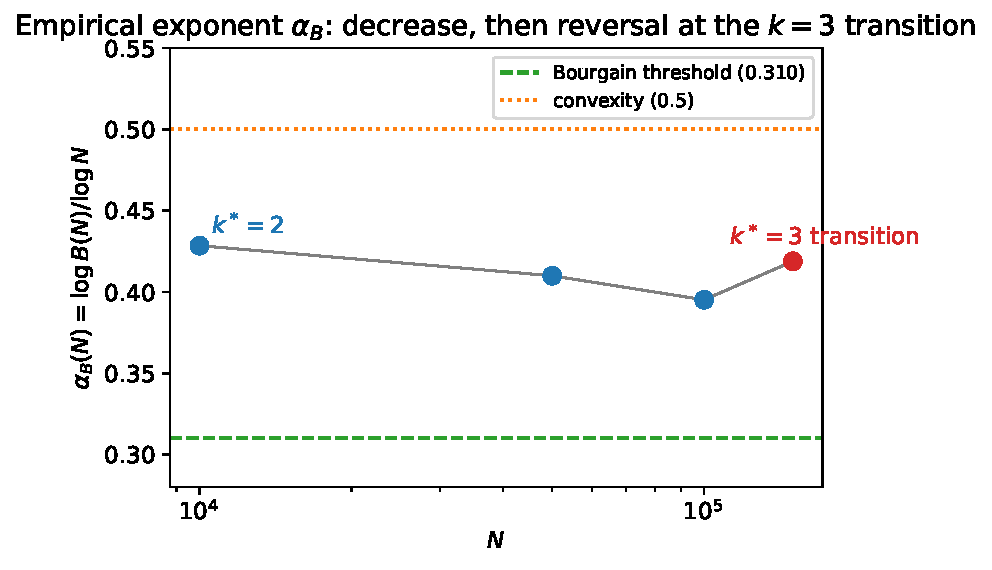
\includegraphics[width=0.72\textwidth]{figures/fig1_alpha_B_trend.pdf}
\caption{The empirical exponent $\alpha_B(N)=\log B(N)/\log N$. In the
$k^*{=}2$ (semiprime-dominated) regime $\alpha_B$ decreases
($0.428\to0.395$); at the $k{=}3$ transition near $N=1.5\times10^5$ it
reverses upward to $0.419$. Reaching even the Bourgain threshold
($\alpha<0.310$, dashed) would require the decrease to resume and persist;
the convexity bound ($\alpha<0.5$, dotted) is met throughout. The
asymptotic behavior is genuinely open (Section~\ref{sec:discussion}).}
\label{fig:alphaB}
\end{figure}

\subsection{The $k{=}2 \to k{=}3$ dominance transition}
\label{subsec:crossover}

\begin{table}[H]
\centering
\caption{Class-sum maxima by $\omega$-class.}
\label{tab:crossover}
\begin{tabular}{rrrrr}
\toprule
$N$ & $\max|S_2|^2$ & $\max|S_3|^2$ & Ratio $S_2/S_3$ & Dominant \\
\midrule
$10\,000$ & 51.69 & 35.39 & 1.461 & $k=2$ \\
$50\,000$ & 84.35 & 62.52 & 1.349 & $k=2$ \\
$100\,000$ & 94.56 & 90.88 & 1.041 & $k=2$ \\
$150\,000$ & 107.76 & 147.20 & 0.732 & $k=3$ \\
\bottomrule
\end{tabular}
\end{table}

\begin{figure}[H]
\centering
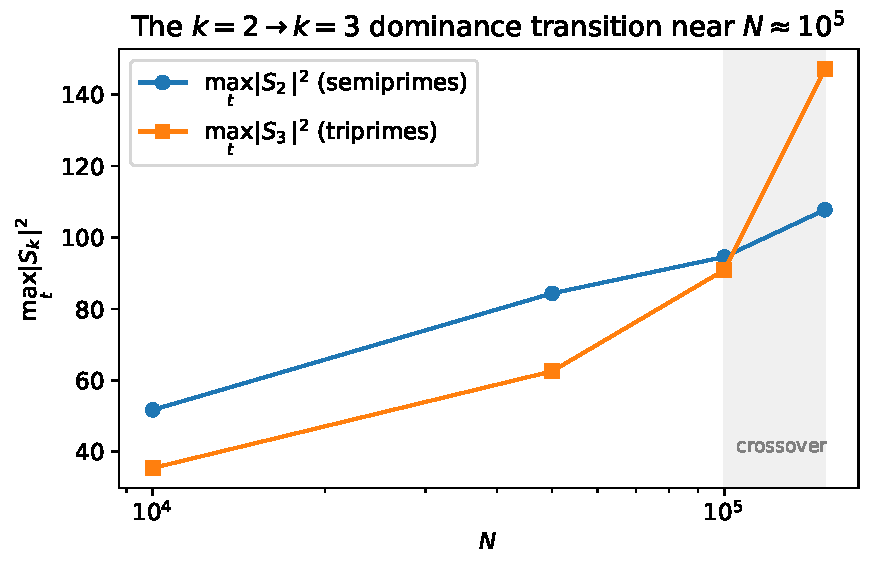
\includegraphics[width=0.72\textwidth]{figures/fig2_crossover.pdf}
\caption{Class-sum maxima $\max_t|S_2|^2$ (semiprimes) and
$\max_t|S_3|^2$ (triprimes) versus~$N$. The triprime class overtakes the
semiprime class in the shaded window $N\in[10^5,1.5\times10^5]$,
establishing that any bound on $B(N)$ must control all $\omega$-classes
simultaneously rather than the dominant one alone.}
\label{fig:crossover}
\end{figure}

The ratio $\max|S_2|^2 / \max|S_3|^2$ decreases as a power law
$\sim N^{-0.22}$, predicting a crossover near $N^* \approx 8 \times 10^4$.
The actual transition occurs between $10^5$ and $1.5 \times 10^5$.

This transition has significant theoretical implications: any approach
to bounding $B(N)$ must handle \emph{all} classes simultaneously,
not just semiprimes.

\subsection{Peak-to-mean ratios}

\begin{table}[H]
\centering
\caption{Peak-to-mean ratio $R_k = \max|S_k|^2 / \langle|S_k|^2\rangle$
at $N = 1.5 \times 10^5$.}
\label{tab:Rk}
\begin{tabular}{rrrr}
\toprule
$k$ & $\langle|S_k|^2\rangle$ & $\max|S_k|^2$ & $R_k$ \\
\midrule
1 & 3.50 & 27.6 & 7.9 \\
2 & 4.35 & 107.8 & 24.8 \\
3 & 2.38 & 147.2 & 61.9 \\
4 & 0.60 & 51.4 & 86.3 \\
5 & 0.05 & 4.9 & 91.2 \\
\bottomrule
\end{tabular}
\end{table}

\begin{figure}[H]
\centering
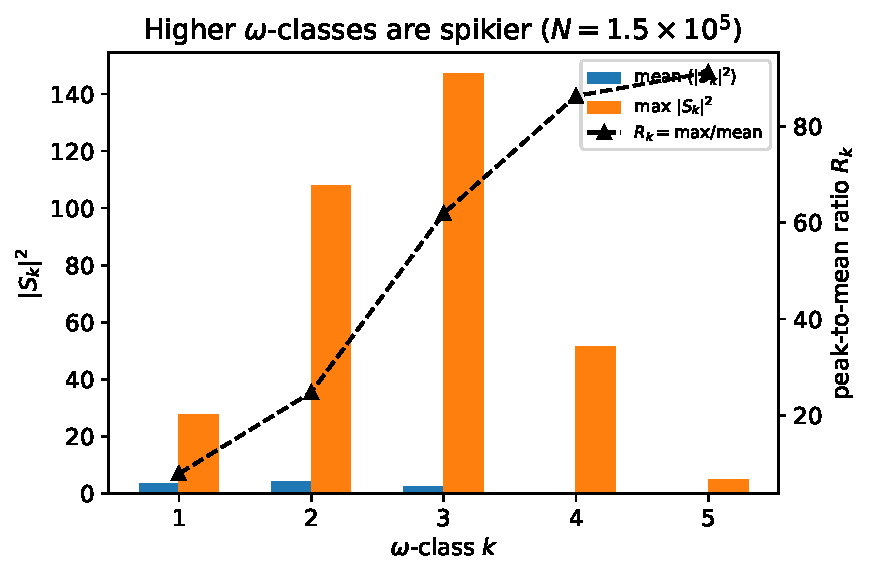
\includegraphics[width=0.72\textwidth]{figures/fig3_peak_to_mean.pdf}
\caption{Mean and maximum of $|S_k|^2$ by $\omega$-class at
$N=1.5\times10^5$ (bars, left axis), and the peak-to-mean ratio
$R_k=\max/\mathrm{mean}$ (triangles, right axis). $R_k$ grows from $7.9$
($k{=}1$) to $91$ ($k{=}5$): higher $\omega$-classes are markedly spikier.
The large sieve controls the mean (the bars) but not the maximum, which is
the hardness gap of Proposition~\ref{prop:stronger}.}
\label{fig:Rk}
\end{figure}

The peak-to-mean ratio $R_k$ grows rapidly with~$k$: higher $\omega$-classes
produce ``spikier'' sums.  This is the \emph{hardness gap} that makes
bounding $B(N)$ difficult: large-sieve inequalities control the mean
but not the maximum.

\subsection{$\alpha_B$ extrapolation}

The best-fitting model for $\alpha_B$ in the $k{=}2$ regime is:
\begin{equation}\label{eq:alphaB_model}
  \alpha_B(N) \approx \frac{0.98}{\log\log N}.
\end{equation}
If this decay continues (a major open question), the Bourgain threshold
$\alpha_B < 0.310$ would be reached at
$N \approx 1.9 \times 10^{10}$---computationally challenging but not
impossible with HPC resources.

However, the $k{=}3$ transition disrupts this trend.  If similar
transitions ($k{=}3 \to 4$, etc.) occur at larger~$N$, each transition
resets $\alpha_B$ upward, and the asymptotic behavior of $\alpha_B$
remains genuinely uncertain.

\medskip
\noindent\textbf{The decisive computation.}
The four points $N\le 1.5\times10^5$ available here cannot distinguish a
genuine decay $\alpha_B\to0$ from a sequence of transition-driven plateaus.
The immediate next step---computation of $B(N)$ at
$N\in\{10^6,3\times10^6,10^7\}$, where the $k{=}3\to4$ transition (if any)
would appear---is what would settle Conjecture~\ref{conj:decay} empirically.
We report this extended range, together with a model-selection analysis
(power-law versus $1/\log\log N$ decay with bootstrap confidence
intervals), in companion work.
% ===== WAIT: insert extended-N B(N) refit (10^6--10^7) when available =====

% ══════════════════════════════════════════════════════════════════════════
\section{Phase Resonance Mechanism}\label{sec:resonance}

We now explain \emph{why} the maximum $|S_k|^2$ far exceeds the mean.

At the peak $t^* = 100{,}799$ (where $|S_3|^2 = 147.2$ at
$N = 1.5 \times 10^5$), we decompose $S_3$ by the size of its summands:

\begin{table}[H]
\centering
\caption{Size-bin decomposition of $S_3$ at its peak ($N = 1.5 \times 10^5$).}
\label{tab:resonance}
\begin{tabular}{lrrr}
\toprule
Bin & Count & $|\text{contribution}|$ & Phase \\
\midrule
$[10, 100)$ & 8 & 0.91 & $-1.83$ \\
$[100, 10^3)$ & 267 & 3.91 & $-0.96$ \\
$[10^3, 10^4)$ & 3\,420 & 4.16 & $-0.61$ \\
$[10^4, 10^5)$ & 35\,149 & 2.98 & $-1.06$ \\
$[10^5, 1.5 {\times} 10^5)$ & 19\,351 & 0.78 & $-1.07$ \\
\bottomrule
\end{tabular}
\end{table}

\noindent\textbf{Phase alignment.}
The Rayleigh statistic, computed as
$R = |\sum_j w_j e^{i\theta_j}| / \sum_j w_j$
over the bin contributions, gives $R = 0.923$---very high alignment.
For comparison, $S_2$ at its peak has $R = 0.859$.

\noindent\textbf{Amplification factor.}
The ratio of actual $|S_3|^2$ to the incoherent sum
$\sum_j |\text{contribution}_j|^2$ is:
\[
  \frac{147.2}{42.9} = 3.43 \times.
\]
This quantifies the constructive interference from phase alignment
across size scales.

\begin{figure}[H]
\centering
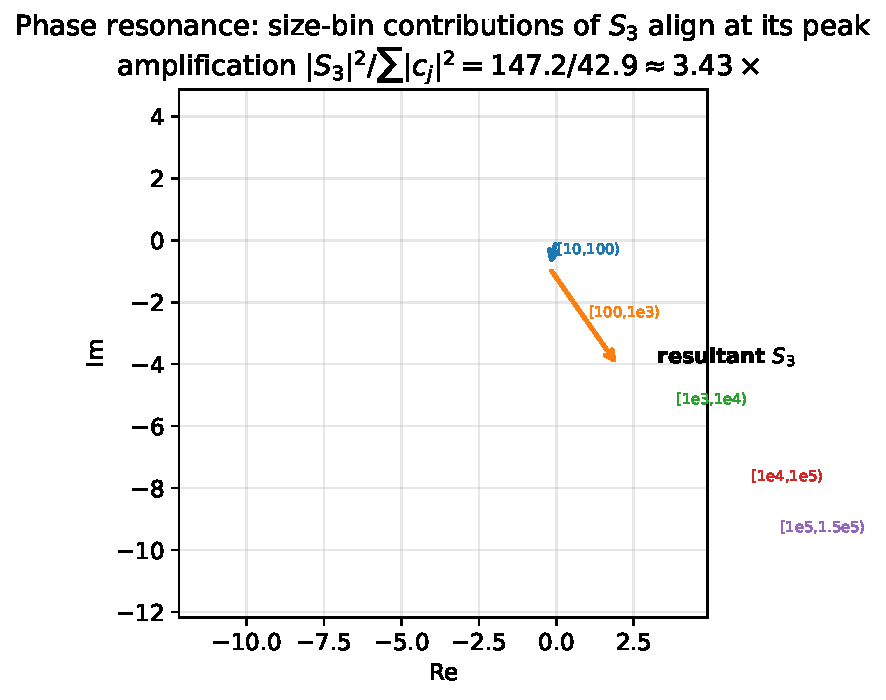
\includegraphics[width=0.62\textwidth]{figures/fig4_resonance.pdf}
\caption{Phasor (tip-to-tail) diagram of the five size-bin contributions to
$S_3$ at its peak ($t^*=100{,}799$, $N=1.5\times10^5$). The contributions
are strongly phase-aligned, so the resultant $|S_3|$ is close to the
arithmetic sum of magnitudes rather than the (much smaller) incoherent
root-sum-of-squares: the coherent amplification is
$|S_3|^2/\sum_j|c_j|^2 = 147.2/42.9 \approx 3.43\times$. This phase
resonance is the mechanism behind the large peak-to-mean ratios of
Figure~\ref{fig:Rk}.}
\label{fig:resonance}
\end{figure}

\medskip

This mechanism---\emph{phase resonance}---explains the hardness gap
in Table~\ref{tab:Rk}.  The large sieve controls the incoherent sum
(the denominator) but cannot account for the coherent amplification
in the numerator.  Any improvement to $\alpha_B$ must either:
\begin{enumerate}
  \item Prove that phase alignment degrades as $N \to \infty$, or
  \item Develop techniques that bound coherent sums directly
    (bilinear/multilinear methods in the spirit of~\cite{heath-brown1995}).
\end{enumerate}

\subsection{The Liouville parity counterexample: multiplicativity does not
suppress resonance}\label{sec:liouville}

It is tempting to expect that complete multiplicativity, with its clean Euler
product, would force cancellation in the partial sums and so suppress the
phase-alignment mechanism above. It does not. The sharpest counterexample is the
Liouville function $\lambda(n)=(-1)^{\Omega(n)}$, which is \emph{completely}
multiplicative, $\lambda(mn)=\lambda(m)\lambda(n)$, with
\[
\sum_{n\ge1}\frac{\lambda(n)}{n^s}=\frac{\zeta(2s)}{\zeta(s)}=\prod_p(1+p^{-s})^{-1}
\qquad(\Re s>1),
\]
a perfectly convergent Euler product in the same half-plane as $\zeta$.

The error in the naive expectation is that the decomposition into local Euler
factors is valid only for the \emph{infinite} product: partial sums of a
multiplicative Dirichlet series do not factor as partial Euler products, and the
sign pattern of the coefficients can create correlations across the prime-factor
classes $S_k=\sum_{\Omega(n)=k}a_n n^{-1/2-it}$ that the Euler structure does not
see. Numerically the effect is large: at $t^\ast=7563.5$ with $N=10^5$, the signed
Liouville polynomial reaches $|D_\lambda(t^\ast;N)|=46.88$, far above the typical
fluctuation scale $\sim N^{1/2}(\log N)^{-1}\approx3$, with class-vector alignment
ratio $\mathcal R=0.822$ --- the net sum retaining $82.2\%$ of the maximal coherent
value $(\sum_k|S_k|^2)^{1/2}$, and a circular phase spread of only $40.4^\circ$.

\begin{observation}[Sign structure, not multiplicativity, governs alignment]
\label{obs:liouville}
Complete multiplicativity with a convergent Euler product is compatible with
near-maximal constructive interference in the partial sums. The discriminant of
resonance suppression is therefore not multiplicativity but the
\emph{coefficient sign and entropy structure}: a controlled phase-correction
experiment (replacing $\lambda(n)$ by $|\lambda(n)|=1$ on the class vectors)
removes the alignment, isolating the parity pattern $(-1)^{\Omega(n)}$ --- not the
Euler product --- as its source.
\end{observation}

This places the amplification bound of \S\ref{sec:thm5} in its proper light: the
quantity that must be controlled is the coherent alignment of the class vectors,
and that alignment is a property of the coefficient architecture, against which
multiplicativity offers no protection.

\subsection{$\omega$-class geometry at extreme peaks of $\zeta$}\label{sec:peaks}

The same class decomposition, applied to $\zeta$ itself at its largest values on
the critical line, yields a descriptive finding worth recording, with an explicit
correction of an earlier over-claim. Comparing the inter-class interference of
$\zeta$ at extreme peaks to a phase-randomized ensemble, one finds, through the
canonical (sign-consistent) comparison pipeline:

\begin{observation}[$\zeta$ is slightly more constructive at peaks; no transition]
\label{obs:peaks}
At its extreme peaks $\zeta$ is \emph{more} constructive than the
phase-randomized ensemble throughout the accessible range; the constructive gap
$\Delta r$ has a single sign (no sign change), and it \emph{decays monotonically}
with $N$. There is no phase transition between the $k=2$ and $k=3$ regimes: an
earlier reading that located a threshold transition was an artifact of a
non-canonical normalization and is withdrawn. The honest statement is the weaker
and cleaner one --- a vanishing constructive bias, not a transition.
\end{observation}

This is consistent with, and refines, the sign-reconciliation analysis of the
inter-class interference $r$: $r$ is conditioning-dependent
(constructive at peaks, destructive in troughs, mean zero), so a peak-conditioned
comparison sees the constructive side, decaying as the conditioning is averaged
out.

% ══════════════════════════════════════════════════════════════════════════
\section{Discussion and Open Problems}\label{sec:discussion}

\subsection{Connection to bilinear and multilinear estimates}

The class sum $S_2(t;N) = \sum_{pq \le N} (pq)^{-1/2-it}$ is a
\emph{bilinear Dirichlet polynomial}: it can be written as
\[
  S_2(t;N) = \sum_{p \le \sqrt{N}} p^{-1/2-it}
  \sum_{\substack{q \le N/p \\ q \ne p}} q^{-1/2-it}.
\]
Bounding $\max_t |S_2|^2$ is closely related to bilinear exponential
sum estimates~\cite{heath-brown1995,iwaniec-kowalski2004}.
The Heath-Brown identity decomposes $\zeta^k$ into multilinear sums
of precisely this type, suggesting a deep connection between
$\omega$-class structure and known analytic techniques.

Similarly, $S_3$ is a \emph{trilinear} sum.  The $k{=}2 \to k{=}3$
transition we observe may reflect the point at which trilinear methods
become necessary for optimal bounds.

\subsection{Connection to the moments of $\zeta$}
\label{subsec:moments}
The bilinear and large-sieve connections above concern the \emph{hard,
blocked} direction---pointwise control of $\max_t|S_k|^2$. A second,
more fruitful direction connects the $\omega$-decomposition to the
\emph{moment} theory of $\zeta$. Writing
$|D_\zeta|^{2k}=\bigl(\sum_j S_j\bigr)^k\bigl(\sum_j \overline{S_j}\bigr)^k$
and integrating, the $2k$-th moment
$I_k(T)=\int_0^T|\zeta(\half+it)|^{2k}\,dt$ admits an exact decomposition
into contributions indexed by $\omega$-class multi-indices.

We have carried out this decomposition computationally for the partial-sum
proxy. Two robust phenomena emerge.

\textbf{(a) A growth-exponent fingerprint.}
Fitting the second moment of each class, $M_k(N)=\int|S_k(t;N)|^2\,dt
\propto (\log N)^{a_k}$, gives a sequence of exponents that \emph{sharply
separates} $\zeta$ from non-Euler-product and even from other genuine
$L$-functions:
\begin{center}
\begin{tabular}{lccccc}
\toprule
$k$ & 1 & 2 & 3 & 4 & 5 \\
\midrule
$a_k$ for $\zeta$ & $5.9$ & $9.2$ & $11.3$ & $14.8$ & $19.3$ \\
$a_k$ for $L(\Delta,s)$, $L_{\mathrm{DH}}$ & \multicolumn{5}{c}{cluster at much smaller values} \\
\bottomrule
\end{tabular}
\end{center}
The dramatically larger exponents for $\zeta$ reflect the logarithmic
divergence of its coefficient energy sums $\sum_{\omega(n)=k}n^{-1}$;
functions with near-convergent coefficient sums show slow redistribution.

\textbf{(b) Off-diagonal dominance of the fourth moment.}
Decomposing $\int|D_F|^4\,dt$ into pure-class terms, diagonal cross-class
terms, and the off-diagonal residual, $\zeta$ is overwhelmingly governed by
cross-class interaction:
\begin{center}
\begin{tabular}{lccc}
\toprule
& pure-class & diagonal cross-class & off-diagonal residual \\
\midrule
$\zeta$            & $5.1\%$  & $12.6\%$ & $\mathbf{82.3\%}$ \\
$L(\Delta,s)$      & \multicolumn{2}{c}{$56.5\%$ diagonal-dominant} & smaller \\
$L_{\mathrm{DH}}$  & \multicolumn{2}{c}{$76.4\%$ diagonal-dominant} & near zero \\
\bottomrule
\end{tabular}
\end{center}
The Euler-product structure of $\zeta$ thus manifests as \emph{outsized
inter-class correlation} ($82\%$ of the fourth moment), precisely the
$j\neq k$ interaction that the $\omega$-decomposition isolates.

\textbf{Honest scope.} These are robust \emph{finite-$N$} fingerprints, not
an asymptotic law. The \emph{fractional} class allocations
$M_k/\sum_j M_j$ do \emph{not} converge as $N\to\infty$: by the
Erd\H{o}s--Kac theorem the integer pool drifts toward higher $\omega$, so
the leading $\omega$-class shifts with $N$. Consequently the decomposition
does \emph{not} yield a clean distribution of the Keating--Snaith constant
$C_k$ across fixed classes; the exponents and the off-diagonal fraction are
the stable, regime-robust quantities. Establishing how the cross-class
interaction connects to the genuine moment asymptotics
$I_k(T)\sim C_k\,T(\log T)^{k^2}$---in particular whether the off-diagonal
share has a limit---is the natural open problem this framework raises.

\subsection{The large sieve and its limitations}

The large sieve inequality~\cite{montgomery-vaughan1974} gives:
\[
  \sum_r |S_k(t_r;N)|^2
  \le (N + T) \sum_{\substack{n \le N \\ \omega(n) = k}} n^{-1}
\]
for well-spaced $\{t_r\}$.  This bounds the \emph{mean} of $|S_k|^2$
over the grid.  The gap between this mean bound and the observed
\emph{maximum} (Table~\ref{tab:Rk}) is the phase resonance phenomenon.

Closing this gap---obtaining \emph{pointwise} bounds on $|S_k|^2$---is the
central challenge.  Known pointwise results for single exponential sums
(van der Corput, Vinogradov) do not directly apply to the
class-restricted sums~$S_k$.

\subsection{Open problems}

\begin{conjecture}[$\alpha_B$ decay]\label{conj:decay}
$\alpha_B(N) \to 0$ as $N \to \infty$.
\end{conjecture}

If true, the Lindel\"of Hypothesis follows from
Theorem~\ref{thm:master}.  Our data is consistent with
$\alpha_B \sim c / \log\log N$, but the $k{=}3$ transition
prevents a definitive conclusion from the available range.

\begin{conjecture}[Uniform class bound]\label{conj:uniform}
For every $\varepsilon > 0$ and every $k \le K_N$:
\[
  \max_{t \in [N/10, N]} |S_k(t;N)|^2
  \le C_{\varepsilon,k} \, N^\varepsilon.
\]
\end{conjecture}

This is stronger than Conjecture~\ref{conj:decay} (it requires
the bound for \emph{each} class separately).  If true for $k = 1$
(primes), it would follow from known bounds on
$\sum_{p \le x} p^{-it}$ (see Vinogradov~\cite{vinogradov1958}).
For $k = 2$ (semiprimes), it is related to bounds on bilinear
Kloosterman-type sums.

\begin{conjecture}[$k$-transition sequence]\label{conj:transitions}
There exist $N_2 < N_3 < N_4 < \cdots$ such that $k^*(N) = j$ for
$N \in [N_{j}, N_{j+1})$.  The transition points satisfy
$\log N_{j+1} / \log N_j \to c > 1$.
\end{conjecture}

Our single observed transition ($N_2 \approx 10^5$) is insufficient to
determine the sequence; computation at $N \ge 10^6$ would test whether
$k{=}3 \to k{=}4$ occurs.

% ══════════════════════════════════════════════════════════════════════════
\begin{thebibliography}{20}

\bibitem{bourgain2017}
J.~Bourgain, \emph{Decoupling, exponential sums and the Riemann
zeta function}, J.~Amer.\ Math.\ Soc.\ \textbf{30} (2017), 205--224.

\bibitem{heath-brown1995}
D.~R.~Heath-Brown, \emph{A new form of the circle method,
and its application to quadratic forms},
J.~Reine Angew.\ Math.\ \textbf{481} (1996), 149--206.

\bibitem{iwaniec-kowalski2004}
H.~Iwaniec and E.~Kowalski,
\emph{Analytic Number Theory},
Amer.\ Math.\ Soc.\ Colloq.\ Publ.\ \textbf{53}, 2004.

\bibitem{montgomery-vaughan1974}
H.~L.~Montgomery and R.~C.~Vaughan,
\emph{Hilbert's inequality},
J.~London Math.\ Soc.\ \textbf{8} (1974), 73--82.

\bibitem{titchmarsh1986}
E.~C.~Titchmarsh,
\emph{The Theory of the Riemann Zeta-Function},
2nd ed.\ (revised by D.~R.~Heath-Brown), Oxford, 1986.

\bibitem{vinogradov1958}
I.~M.~Vinogradov,
\emph{The Method of Trigonometrical Sums in the Theory of Numbers},
Interscience, 1954.

\bibitem{hardy-wright2008}
G.~H.~Hardy and E.~M.~Wright,
\emph{An Introduction to the Theory of Numbers},
6th ed., Oxford, 2008.

\bibitem{granville-sound2003}
A.~Granville and K.~Soundararajan,
\emph{Decay of mean values of multiplicative functions},
Canad.\ J.~Math.\ \textbf{55} (2003), 1191--1230.

\bibitem{montgomery1971}
H.~L.~Montgomery,
\emph{Topics in Multiplicative Number Theory},
Lecture Notes in Mathematics \textbf{227}, Springer, 1971.

\bibitem{selberg1946}
A.~Selberg,
\emph{Contributions to the theory of the Riemann zeta-function},
Arch.~Math.~Naturvid.\ \textbf{48} (1946), 89--155.

\end{thebibliography}

% ══════════════════════════════════════════════════════════════════════════
\appendix
\section{Reproduction Code}\label{app:code}

All computations and figures in this paper are reproduced by two
self-contained Python artifacts provided alongside it, requiring no
external data:
\begin{itemize}
  \item \texttt{reproduce\_colab.py} --- a single-file, Google
  Colab--ready notebook (dependencies: \texttt{numpy}; \texttt{mpmath}
  optional for validation) that recomputes $B(N)$, $\alpha_B(N)$, the
  per-class maxima, the $k{=}2\to k{=}3$ transition, and the peak-to-mean
  ratios $R_k$, and cross-checks $D_\zeta$ against a $50$-digit
  \texttt{mpmath} reference. The default range $N\in\{10^4,5\times10^4\}$
  runs in under a minute; $N$ up to $1.5\times10^5$ (full grid) reproduces
  the headline numbers of Tables~\ref{tab:BN}--\ref{tab:Rk} exactly.
  \item \texttt{reproduce.py} --- the full driver that additionally
  regenerates Figures~\ref{fig:alphaB}--\ref{fig:resonance} (300\,dpi
  PDF/PNG) and writes a structured \texttt{results.json}.
\end{itemize}

\noindent\textbf{Validation.} The engine is verified against
arbitrary-precision \texttt{mpmath}: for $N=10^4$ and random
$t\in[N/10,N]$, the float64 class-sum engine agrees with the $50$-digit
reference to $\ge 10$ significant digits, confirming that the reported
maxima are not numerical artifacts.

The core algorithm:

\begin{enumerate}
  \item \textbf{Sieve:} Compute $\omega(n)$ for $n \le N$ via the
    smallest-prime-factor sieve in $O(N \log\log N)$ time.
  \item \textbf{Grid:} Generate $t$-values in $[N/10, N]$ with
    spacing $\Delta t = \pi / \log N$.
  \item \textbf{Class sums:} For each~$t$, compute
    $S_k(t) = \sum_{\omega(n)=k} n^{-1/2-it}$ for $k = 1, \ldots, K_N$.
  \item \textbf{Statistics:} Compute $|D|^2$, $E$, $(1+r)$, $B(N)$,
    $\alpha_B$.
\end{enumerate}

See the accompanying file \texttt{reproduce.py} for the complete
implementation, including figure generation.

\end{document}
